In Figure \ref{fig:CfrAverage}, the average correlation distributions from the published analysis in p-Pb 2013 sample (black points) and the new p-Pb 2016 sample (red points), both at 5 TeV, are compared. As it's evident, the statistical and systematic uncertainties are largely reduced ({\bf WARNING: SYST UNCERTAINTIES NOT FINAL FOR 2016, THEY WILL REDUCE}) in the new data sample. The feature of the correlation distributions are the same in both systems, and an overall compatibility of the points is observed. Only in the near-side region, the 2016 points are generally slightly below the 2013 points. In part, this can be partially explained with the different procedure for assessing the B to D decay topology bias (2016 data are corrected, with a slight downward shift for the first two points, while for 2013 data only a downward systematic uncertainty was applied.

\begin{figure}[!htbp]
\centering
%Marianna
\centering
{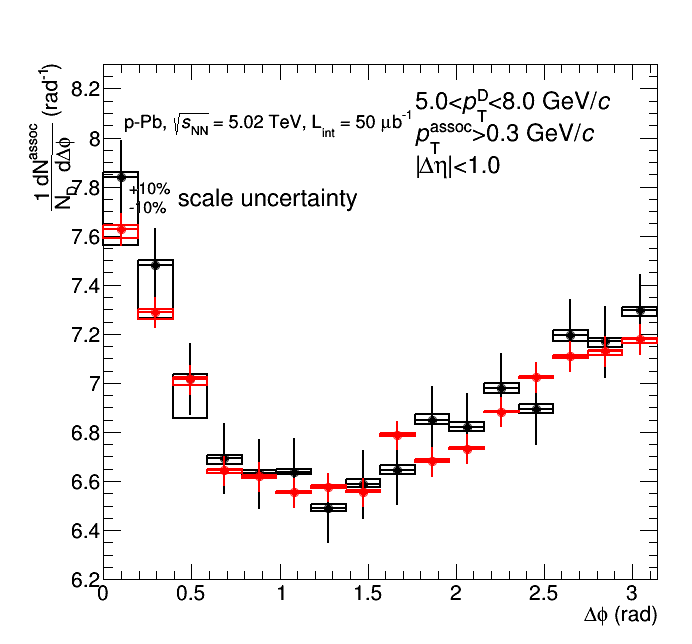
\includegraphics[width=0.47\linewidth]{figures/Cfr2013vs2016/Average_Cfr_2013_2016_Pt5to8_Thr03to99.png}}
{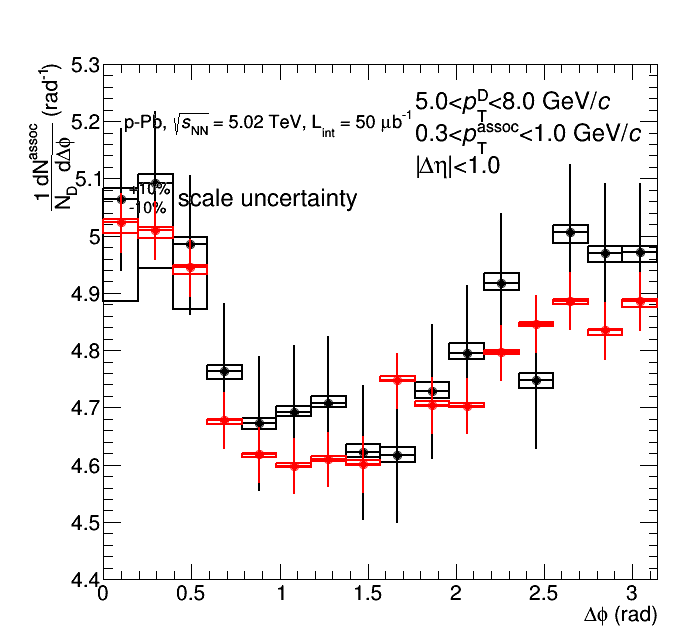
\includegraphics[width=0.47\linewidth]{figures/Cfr2013vs2016/Average_Cfr_2013_2016_Pt5to8_Thr03to1.png}}
{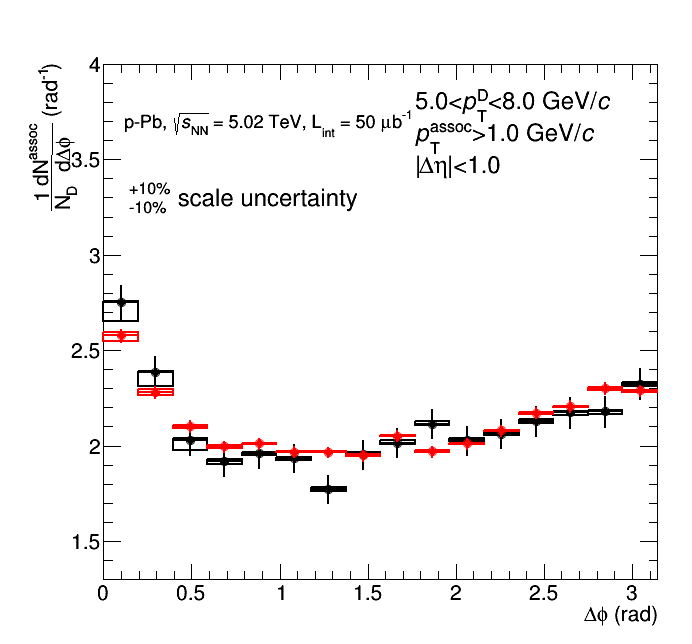
\includegraphics[width=0.47\linewidth]{figures/Cfr2013vs2016/Average_Cfr_2013_2016_Pt5to8_Thr1to99.png}}
{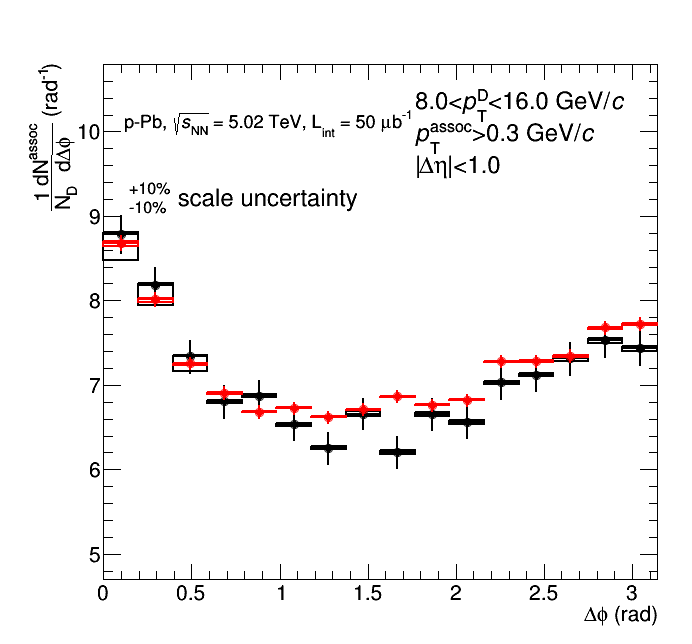
\includegraphics[width=0.47\linewidth]{figures/Cfr2013vs2016/Average_Cfr_2013_2016_Pt8to16_Thr03to99.png}}
{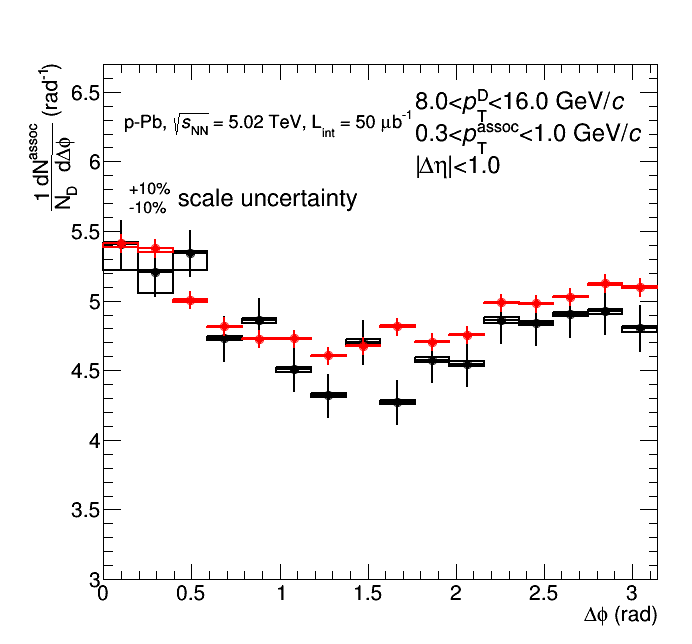
\includegraphics[width=0.47\linewidth]{figures/Cfr2013vs2016/Average_Cfr_2013_2016_Pt8to16_Thr03to1.png}}
{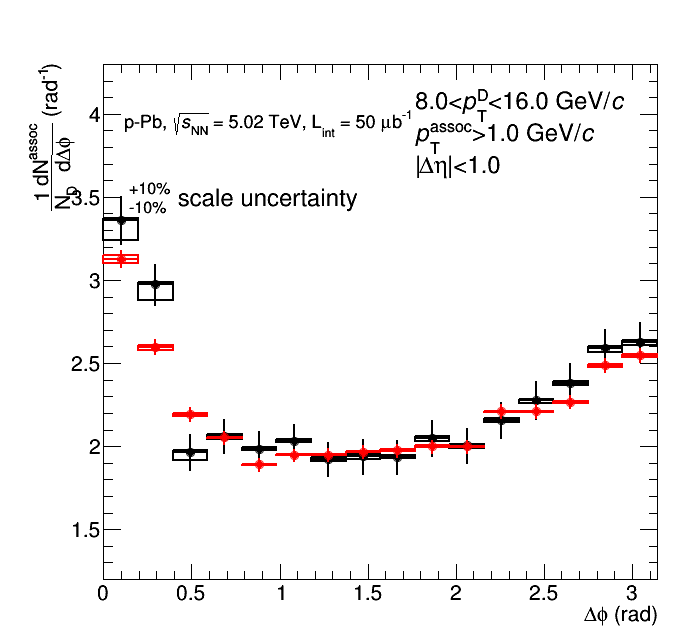
\includegraphics[width=0.47\linewidth]{figures/Cfr2013vs2016/Average_Cfr_2013_2016_Pt8to16_Thr1to99.png}}
\caption{Comparison of 2016 (red) and 2013 (black) results for azimuthal correlation distributions, for the common $\pt$ ranges.}
\label{fig:CfrAverage}
\end{figure}

Figure \ref{fig:CfrObs} shows the same comparison for the fit observables. Also in this case the uncertainties are largely reduced for the 2016 analysis ({\bf WARNING: SYST UNCERTAINTIES NOT FINAL FOR 2016, THEY WILL REDUCE}). While the away side features are compatible (but with large uncertainties) and the near-side widths are on top of each other, for the near-side yields a slight decrease of the 2016 results is observed (though well within the uncertainty). This is a direct consequence of the feature just observed in the comparison of the near-side peak point of the azimuthal correlation distributions.

\begin{figure}[!htbp]
\centering
%Marianna
\centering
{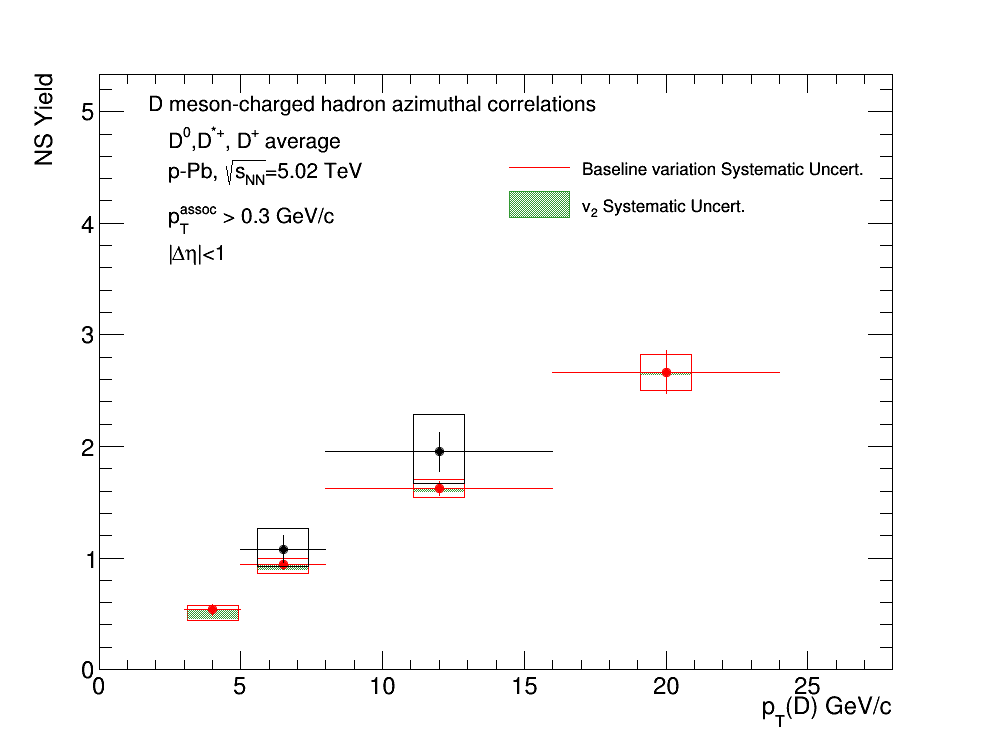
\includegraphics[width=0.31\linewidth]{figures/Cfr2013vs2016/NSYield_Cfr_2013_2016_Thr03to99.png}}
{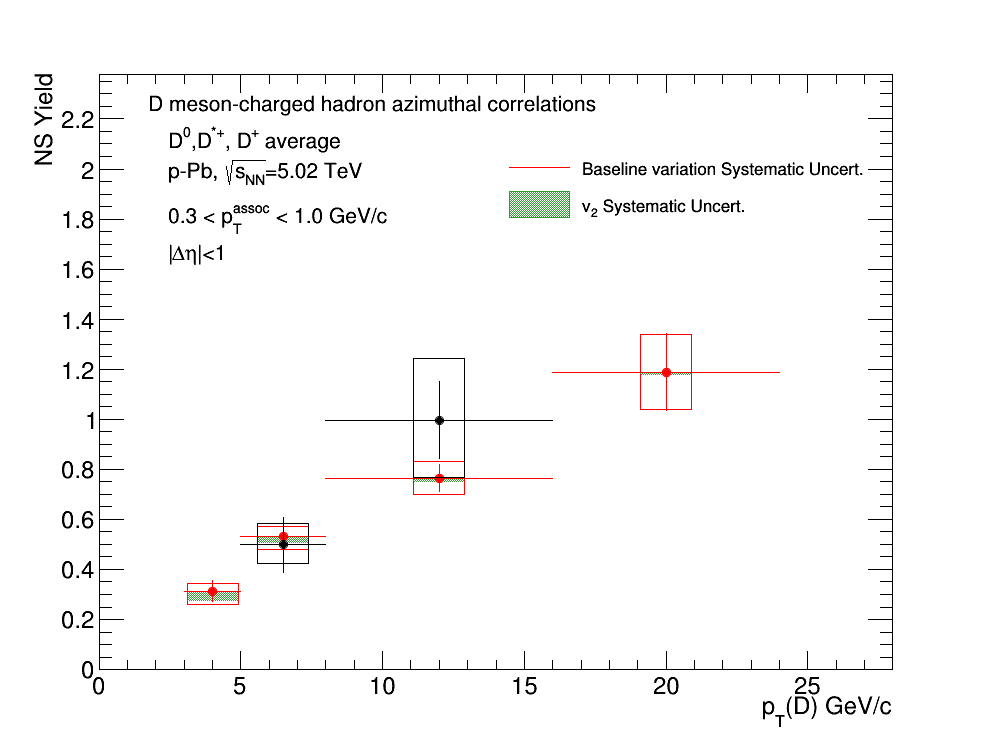
\includegraphics[width=0.31\linewidth]{figures/Cfr2013vs2016/NSYield_Cfr_2013_2016_Thr03to1.png}}
{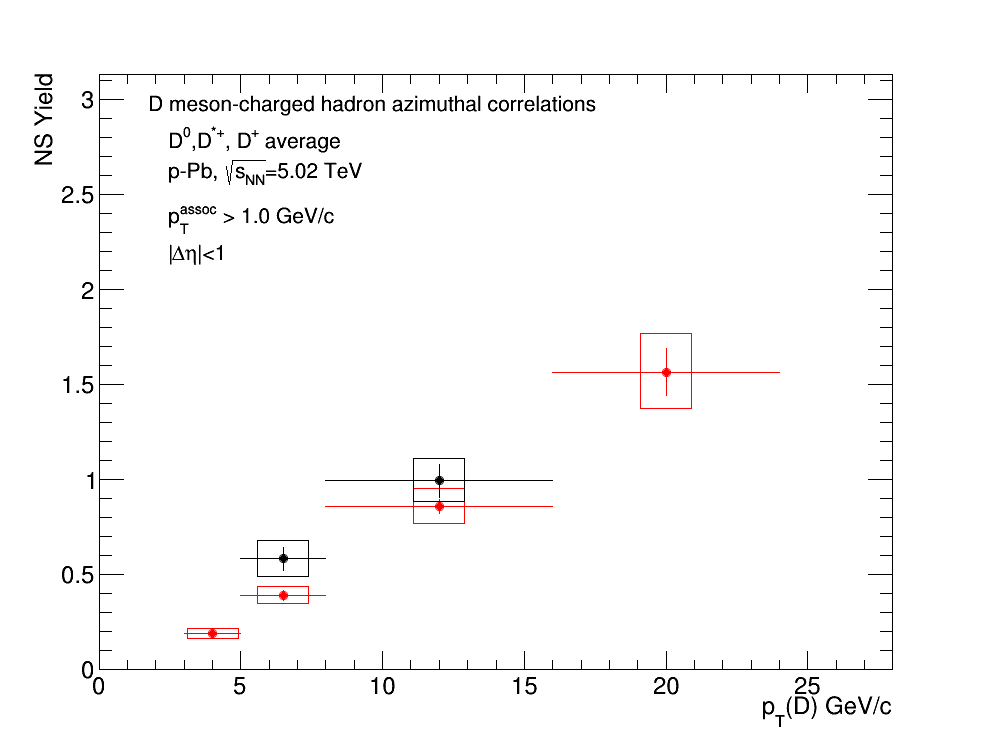
\includegraphics[width=0.31\linewidth]{figures/Cfr2013vs2016/NSYield_Cfr_2013_2016_Thr1to99.png}}
{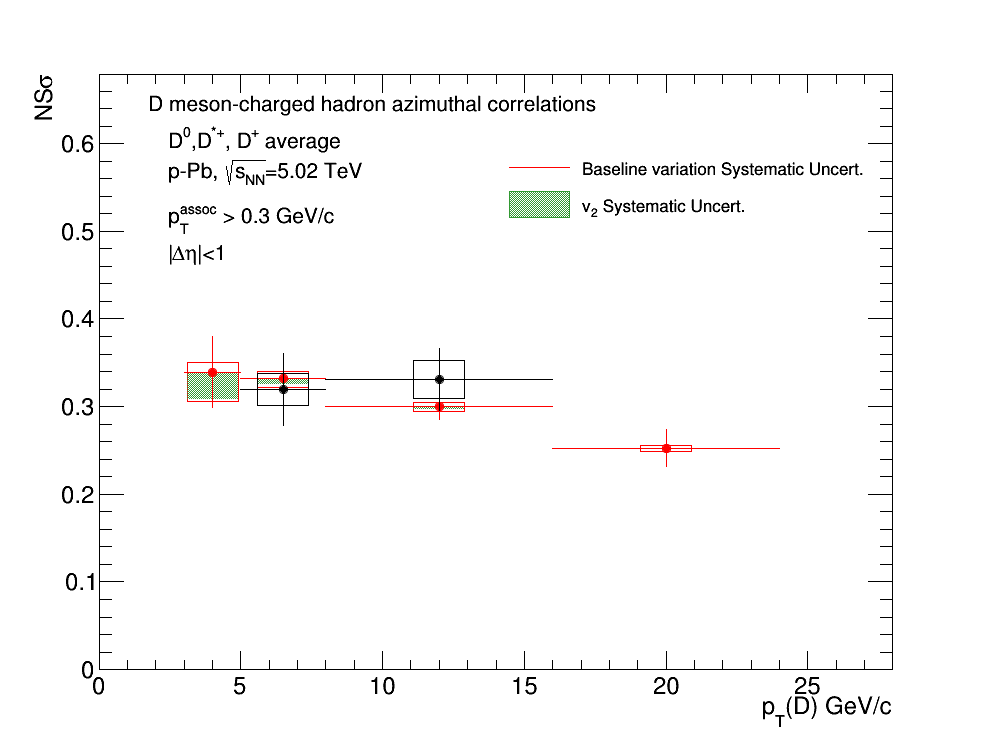
\includegraphics[width=0.31\linewidth]{figures/Cfr2013vs2016/NSsigma_Cfr_2013_2016_Thr03to99.png}}
{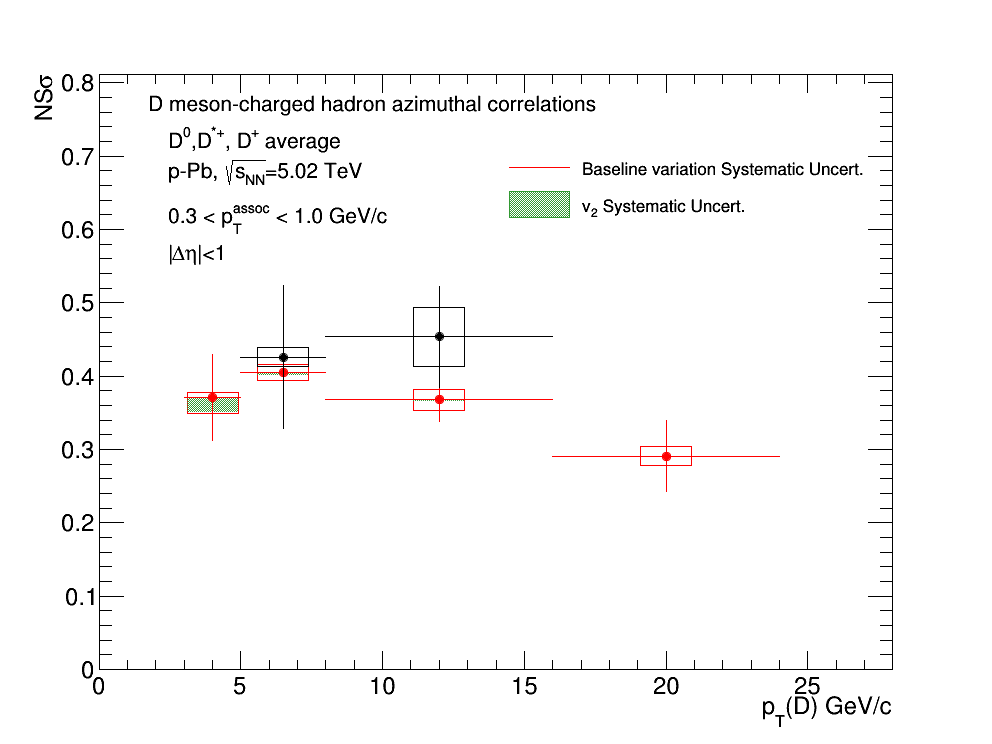
\includegraphics[width=0.31\linewidth]{figures/Cfr2013vs2016/NSsigma_Cfr_2013_2016_Thr03to1.png}}
{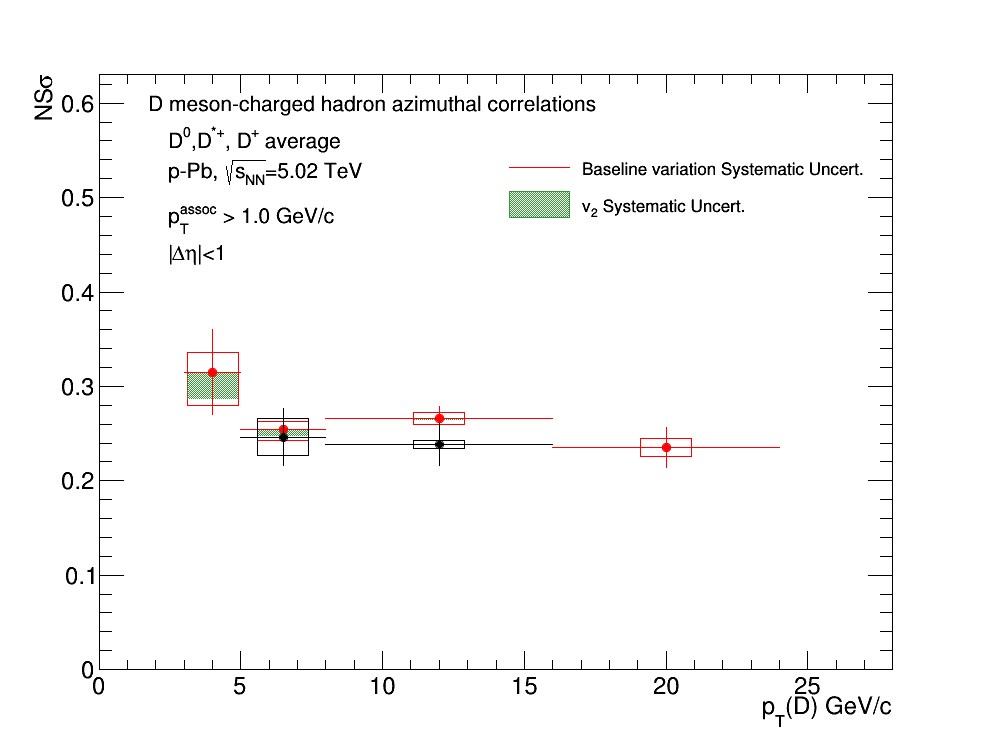
\includegraphics[width=0.31\linewidth]{figures/Cfr2013vs2016/NSsigma_Cfr_2013_2016_Thr1to99.png}}
{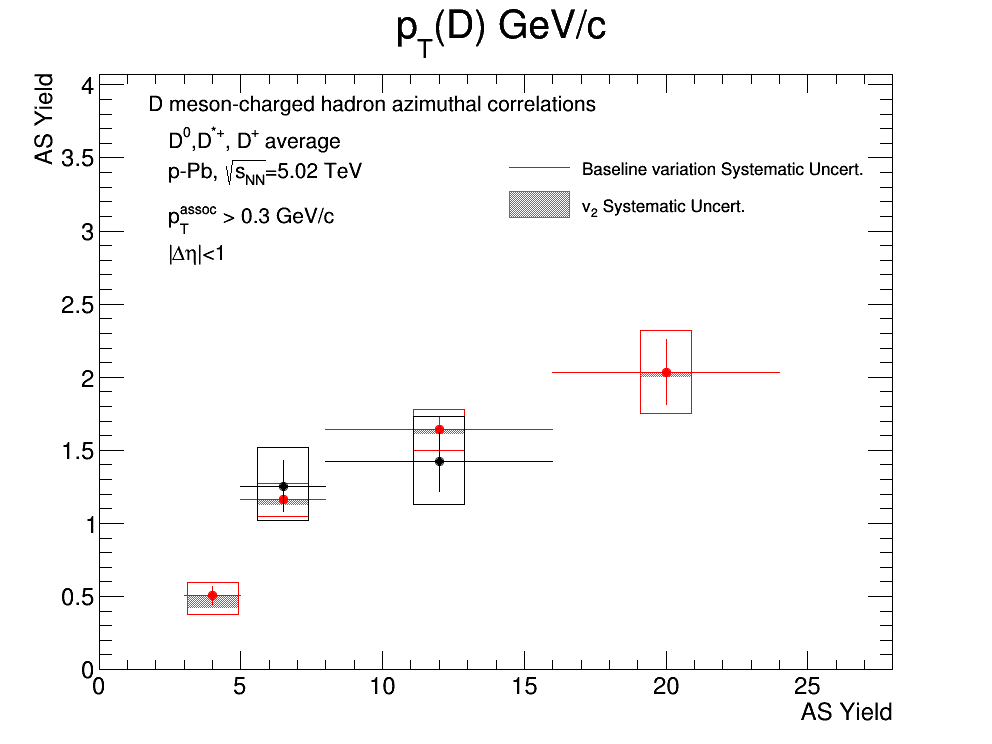
\includegraphics[width=0.31\linewidth]{figures/Cfr2013vs2016/ASYield_Cfr_2013_2016_Thr03to99.png}}
{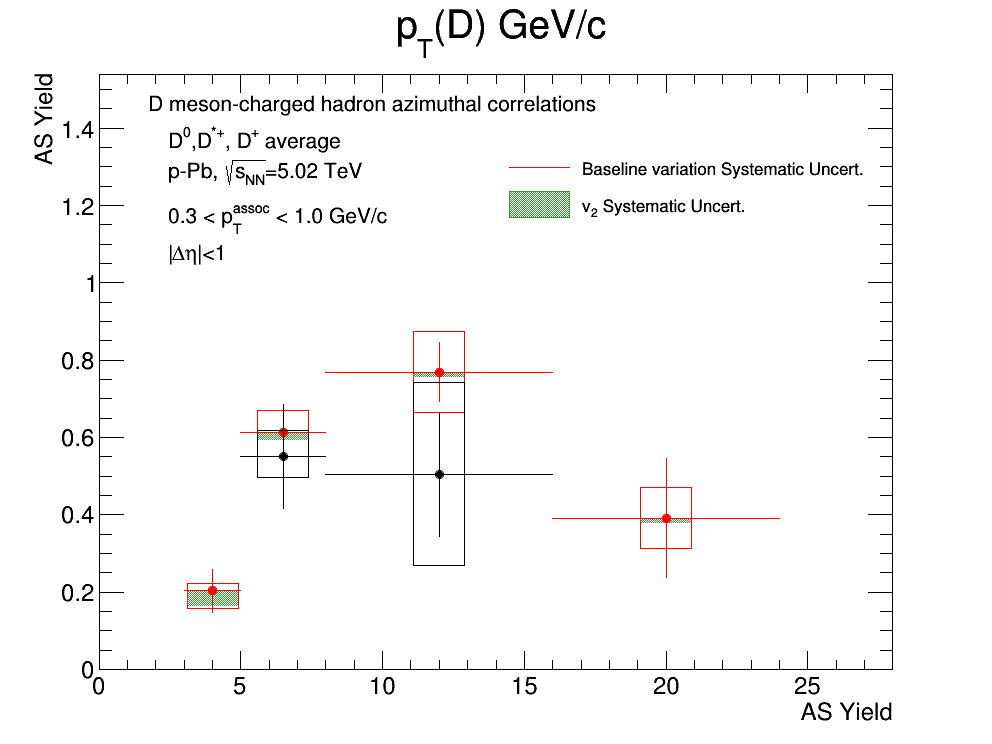
\includegraphics[width=0.31\linewidth]{figures/Cfr2013vs2016/ASYield_Cfr_2013_2016_Thr03to1.png}}
{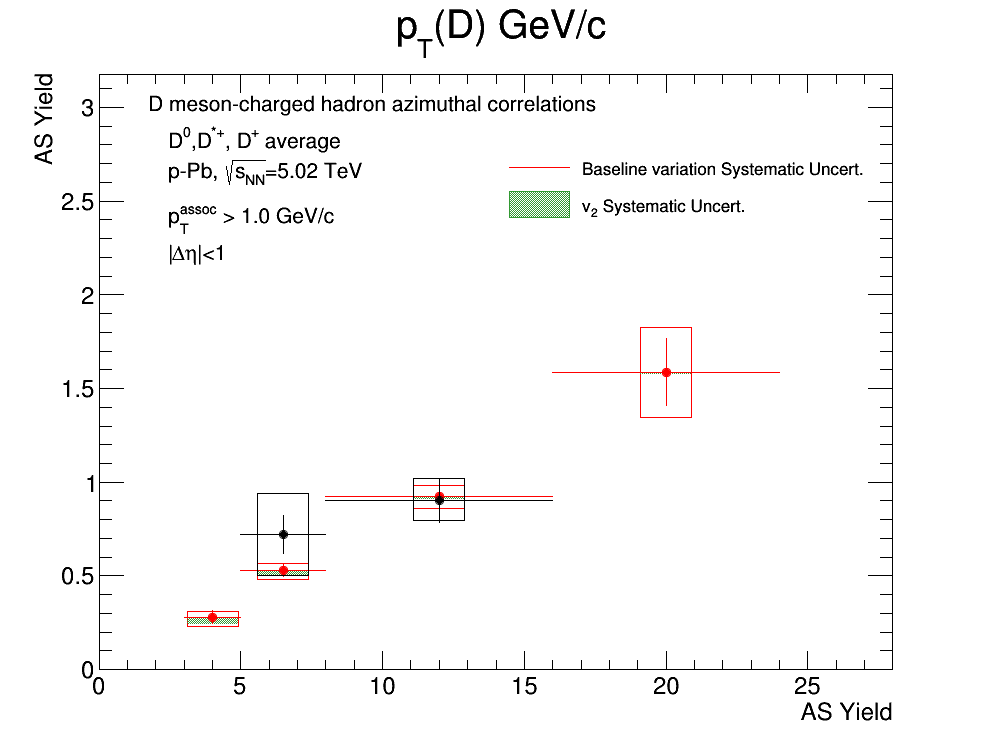
\includegraphics[width=0.31\linewidth]{figures/Cfr2013vs2016/ASYield_Cfr_2013_2016_Thr1to99.png}}
{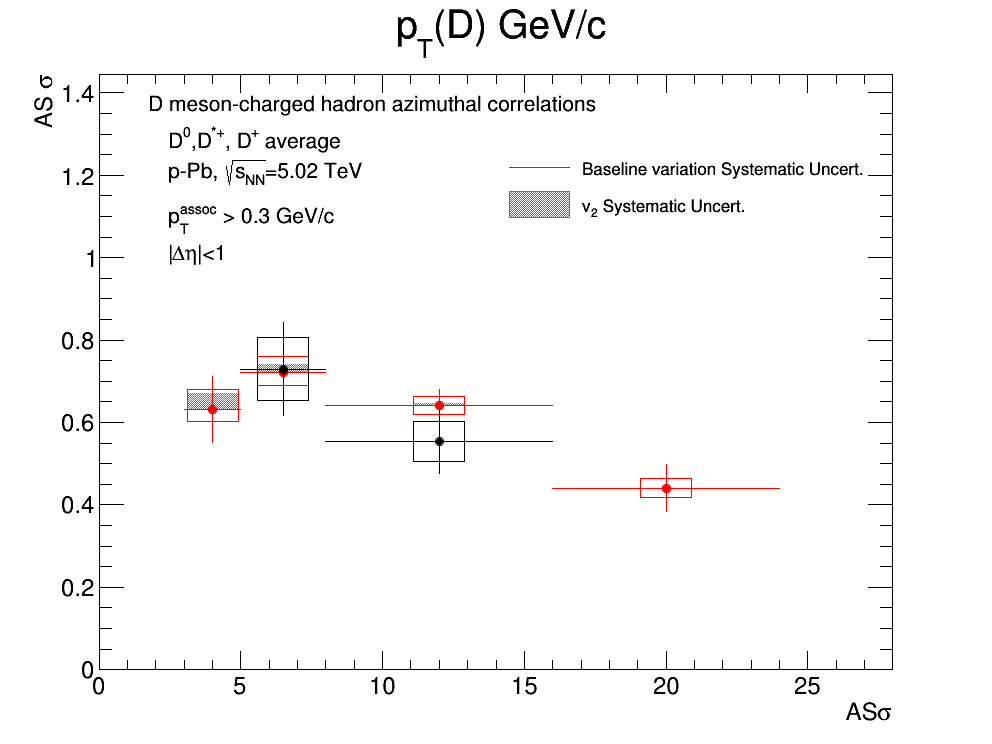
\includegraphics[width=0.31\linewidth]{figures/Cfr2013vs2016/ASsigma_Cfr_2013_2016_Thr03to99.png}}
{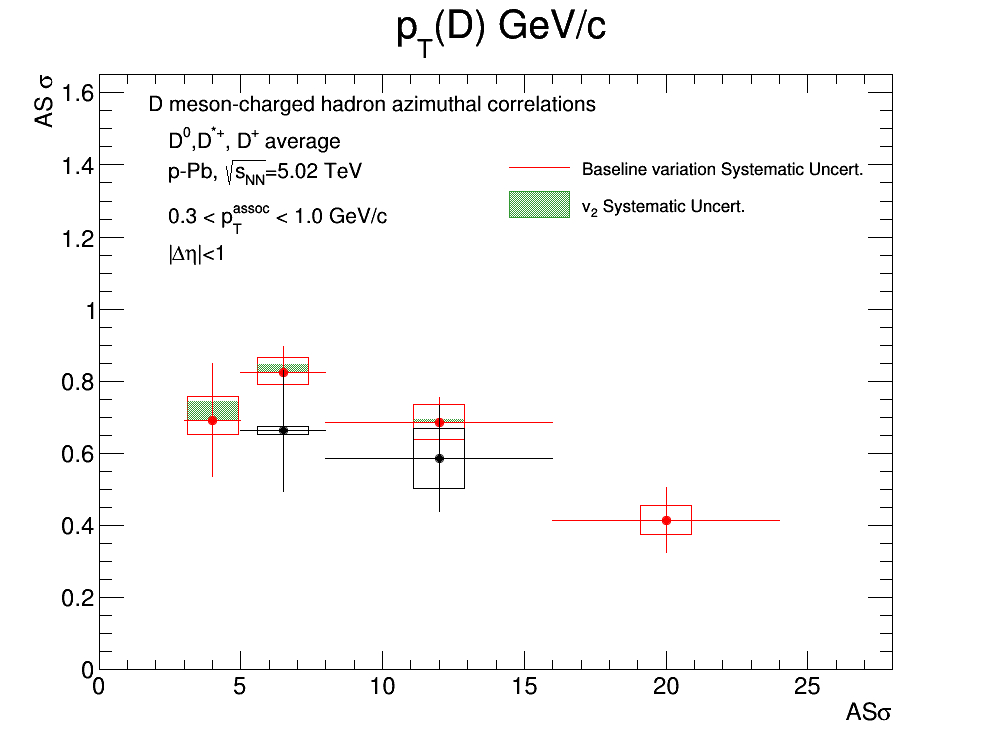
\includegraphics[width=0.31\linewidth]{figures/Cfr2013vs2016/ASsigma_Cfr_2013_2016_Thr03to1.png}}
{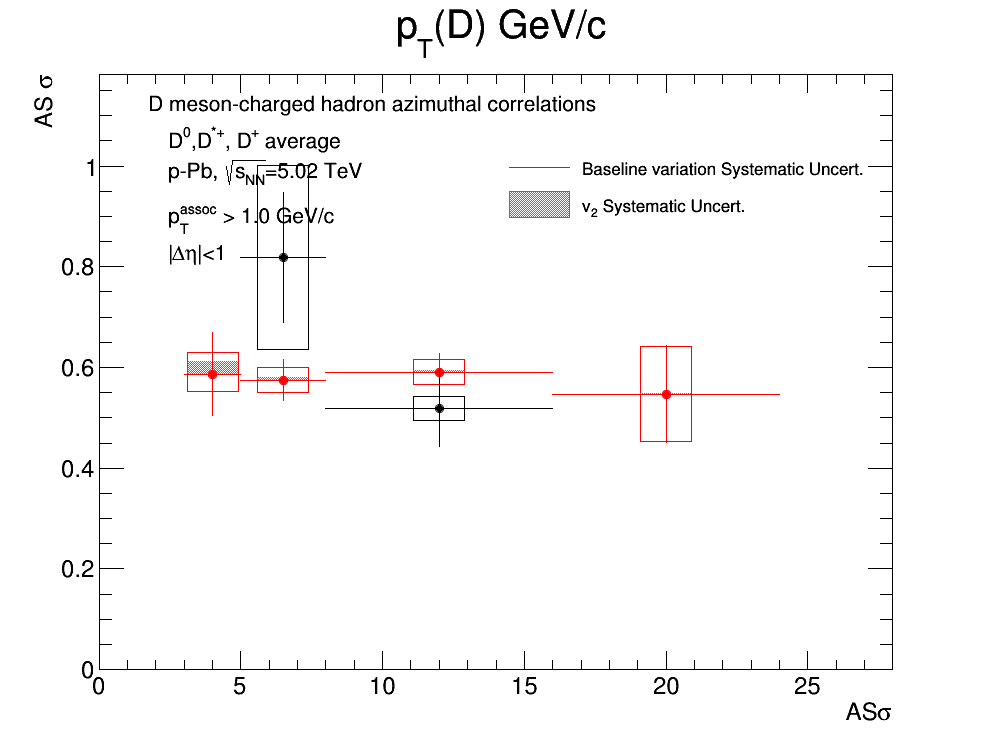
\includegraphics[width=0.31\linewidth]{figures/Cfr2013vs2016/ASsigma_Cfr_2013_2016_Thr1to99.png}}
{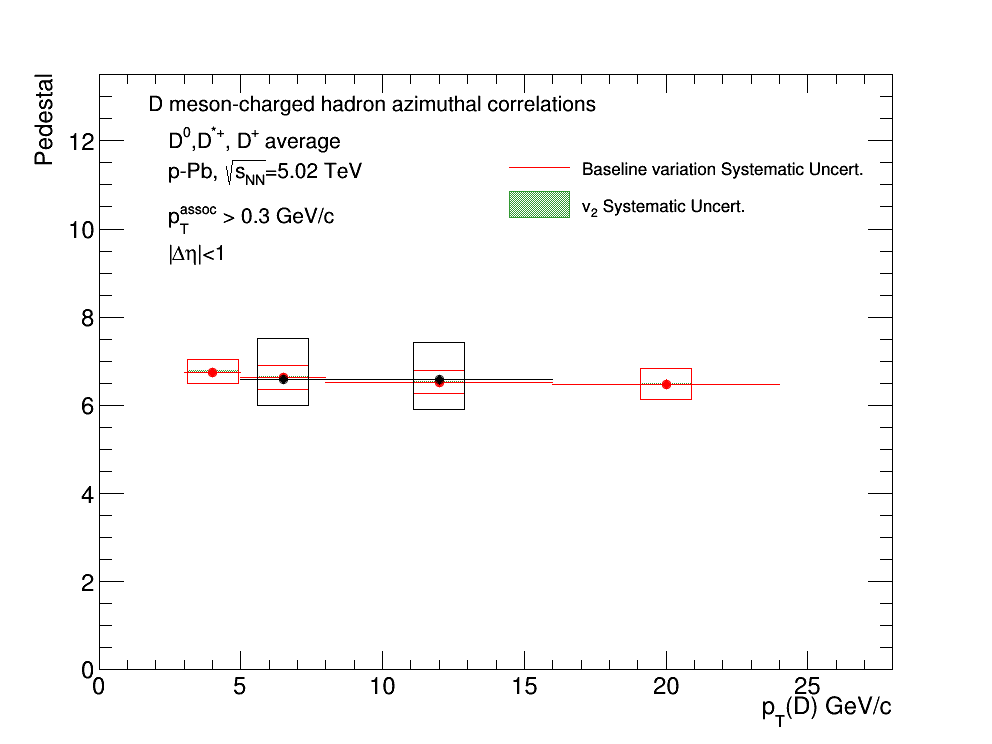
\includegraphics[width=0.31\linewidth]{figures/Cfr2013vs2016/Pedestal_Cfr_2013_2016_Thr03to99.png}}
{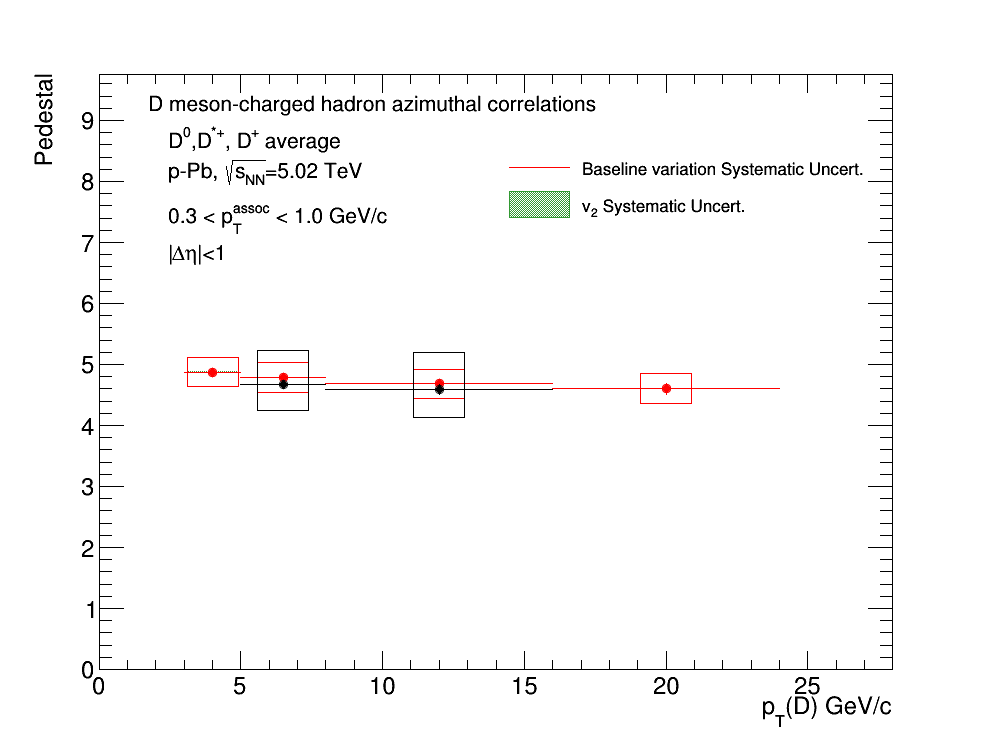
\includegraphics[width=0.31\linewidth]{figures/Cfr2013vs2016/Pedestal_Cfr_2013_2016_Thr03to1.png}}
{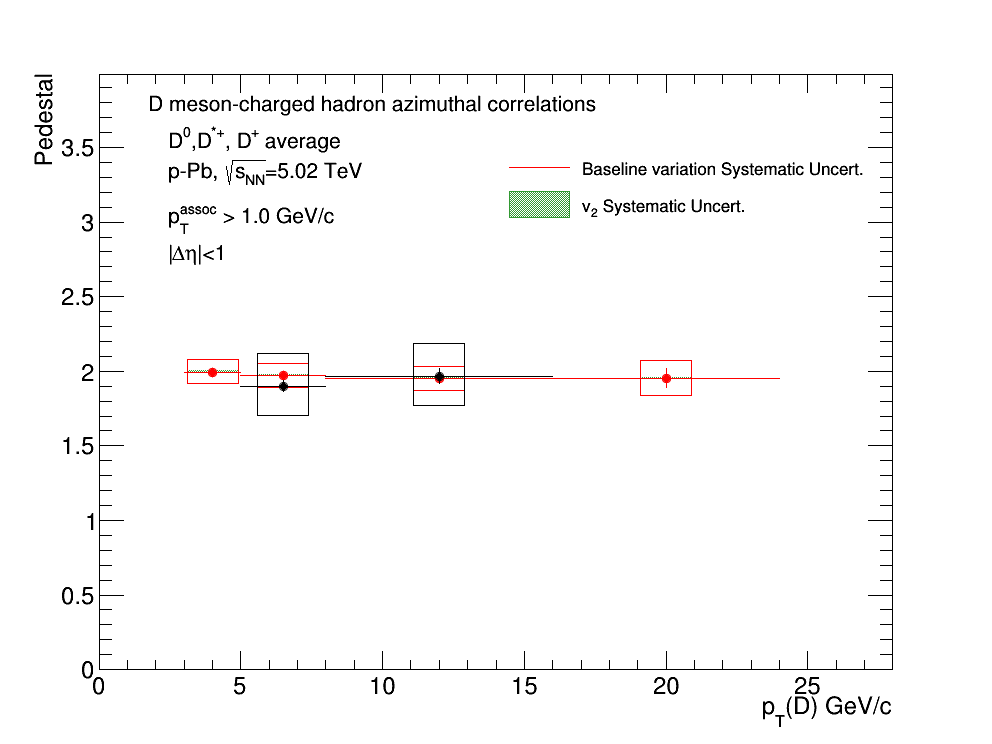
\includegraphics[width=0.31\linewidth]{figures/Cfr2013vs2016/Pedestal_Cfr_2013_2016_Thr1to99.png}}
\caption{Comparison of 2016 (red) and 2013 (black) results for azimuthal correlation distributions, for the common $\pt$ ranges.}
\label{fig:CfrObs}
\end{figure}